\documentclass{beamer}
\mode<presentation>
\usepackage{amsmath}
\usepackage{amssymb}
%\usepackage{advdate}
\usepackage{adjustbox}
\usepackage{subcaption}
\usepackage{enumitem}
\usepackage{multicol}
\usepackage{mathtools}
\usepackage{listings}
\usepackage{url}
\def\UrlBreaks{\do\/\do-}
\usetheme{Boadilla}
\usecolortheme{lily}
\setbeamertemplate{footline}
{
  \leavevmode%
  \hbox{%
  \begin{beamercolorbox}[wd=\paperwidth,ht=2.25ex,dp=1ex,right]{author in head/foot}%
    \insertframenumber{} / \inserttotalframenumber\hspace*{2ex} 
  \end{beamercolorbox}}%
  \vskip0pt%
}
\setbeamertemplate{navigation symbols}{}

\providecommand{\nCr}[2]{\,^{#1}C_{#2}} % nCr
\providecommand{\nPr}[2]{\,^{#1}P_{#2}} % nPr
\providecommand{\mbf}{\mathbf}
\providecommand{\pr}[1]{\ensuremath{\Pr\left(#1\right)}}
\providecommand{\qfunc}[1]{\ensuremath{Q\left(#1\right)}}
\providecommand{\sbrak}[1]{\ensuremath{{}\left[#1\right]}}
\providecommand{\lsbrak}[1]{\ensuremath{{}\left[#1\right.}}
\providecommand{\rsbrak}[1]{\ensuremath{{}\left.#1\right]}}
\providecommand{\brak}[1]{\ensuremath{\left(#1\right)}}
\providecommand{\lbrak}[1]{\ensuremath{\left(#1\right.}}
\providecommand{\rbrak}[1]{\ensuremath{\left.#1\right)}}
\providecommand{\cbrak}[1]{\ensuremath{\left\{#1\right\}}}
\providecommand{\lcbrak}[1]{\ensuremath{\left\{#1\right.}}
\providecommand{\rcbrak}[1]{\ensuremath{\left.#1\right\}}}
\theoremstyle{remark}
\newtheorem{rem}{Remark}
\newcommand{\sgn}{\mathop{\mathrm{sgn}}}
\providecommand{\abs}[1]{\left\vert#1\right\vert}
\providecommand{\res}[1]{\Res\displaylimits_{#1}} 
\providecommand{\norm}[1]{\lVert#1\rVert}
\providecommand{\mtx}[1]{\mathbf{#1}}
\providecommand{\mean}[1]{E\left[ #1 \right]}
\providecommand{\fourier}{\overset{\mathcal{F}}{ \rightleftharpoons}}
%\providecommand{\hilbert}{\overset{\mathcal{H}}{ \rightleftharpoons}}
\providecommand{\system}{\overset{\mathcal{H}}{ \longleftrightarrow}}
	%\newcommand{\solution}[2]{\textbf{Solution:}{#1}}
%\newcommand{\solution}{\noindent \textbf{Solution: }}
\providecommand{\dec}[2]{\ensuremath{\overset{#1}{\underset{#2}{\gtrless}}}}
\newcommand{\myvec}[1]{\ensuremath{\begin{pmatrix}#1\end{pmatrix}}}
\let\vec\mathbf

\lstset{
%language=C,
frame=single, 
breaklines=true,
columns=fullflexible
}

\numberwithin{equation}{section}

\title{Presentation Template}
\author{S A Aravind Eswar - EE24BTECH11053}

\date{\today} 
\begin{document}

\begin{frame}
\titlepage
\end{frame}

\section*{Outline}
\begin{frame}
\tableofcontents
\end{frame}
\section{Problem}
\begin{frame}
\frametitle{Problem Statement}
%
Find the area of region bounded by the curve 
\begin{align}
    x^2 &= 4y\\
    y&=2\\
    y&=4\\
\end{align}
and the y-axis in the first quadrant.
\end{frame}

%\subsection{Literature}
\section{Solution}

\subsection{Finding equation of conic}
\begin{frame}
    \frametitle{Finding equation of conic}

    \begin{align}
        x^2 = 4y\\
        \vec{V} &= \myvec{1 & 0\\ 0 & 0}\\
        \vec{u} &= \myvec{0\\2}
        f &= 0
        g(\vec{x}) &= x^\top\myvec{1 & 0\\0 & 0}\vec{x} + 2\myvec{0\\2}^\top\vec{x} = 0
    \end{align}
\end{frame}

\subsection{Finding points of intersection}
\begin{frame}
\frametitle{Finding points of intersection}
%\framesubtitle{Literature}
Using,
\begin{align}
\kappa_i = \frac{1}{\vec{m}^\top\vec{V}\vec{m}}\brak{-\vec{m}^\top\brak{\vec{Vh}+\vec{u}}\pm\sqrt{\sbrak{\vec{m}^\top\brak{\vec{Vh}+\vec{u}}-g(\vec{h})(\vec{m}^\top\vec{Vm})}}}
\end{align}

and substituing in the line equation ($\vec{x} = \vec{h} - \kappa\vec{m}$)

we get points of intersection,
\begin{align}
a_1 &= \myvec{2\sqrt{2}\\2}\\
a_2 &= \myvec{4\\4}
\end{align}

\end{frame}

\subsection{Plotting the curve}
\begin{frame}
\frametitle{Plotting the curve}
\begin{figure}[h]
    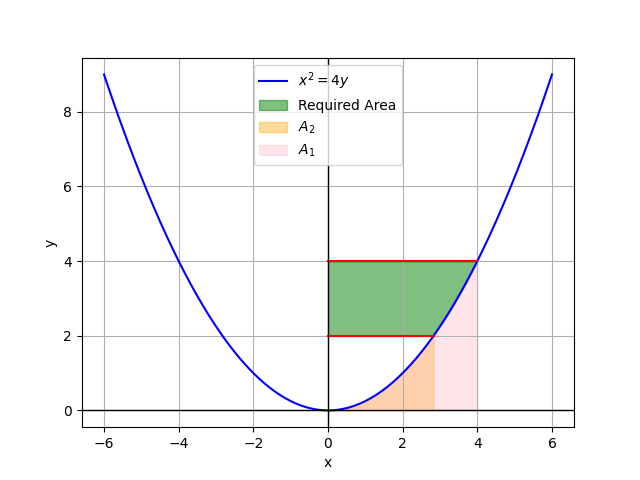
\includegraphics[scale=0.6]{./figs/fig1.png}
\centering
\end{figure}
\end{frame}
%\section{Plot}
\subsection{Integration}
\begin{frame}
\frametitle{Integration}

Calculating $A_1$ and $A_2$,
\begin{align}
A_1 = \int_0^4 \frac{x^2}{4} dx = \frac{16}{3}\\
A_2 = \int_0^{2\sqrt{2}} \frac{x^2}{4} dx = \frac{4\sqrt{2}}{3}
\end{align}

Final area,

\begin{align}
A = \brak{\int_0^4 4 dx - A_1} - \brak{\int_0^{2\sqrt{2}}2 dx - A_2} = \frac{32-8\sqrt{2}}{3}
\end{align}

\end{frame}
\subsection{Code}
\begin{frame}[fragile, allowframebreaks]
    \frametitle{Code}
    Code for generating the points using C:
    \lstset{
        language = C,
        basicstyle=\ttfamily\small,
        keywordstyle=\color{blue},
        stringstyle=\color{green},
        commentstyle=\color{gray},
        tabsize=4
    }
    \lstinputlisting{./codes/points.c}
    
    Code for plotting the graph of the curve and area using Python:
    \lstset{
        language=Python,
        basicstyle=\ttfamily\small,
        keywordstyle=\color{blue},
        stringstyle=\color{green},
        commentstyle=\color{gray},
        tabsize=4
    }
    \lstinputlisting{./codes/plot.py}
\end{frame}
\end{document}
